%!TEX encoding = UTF-8 Unicode
%!TEX root = ../fiche.tex

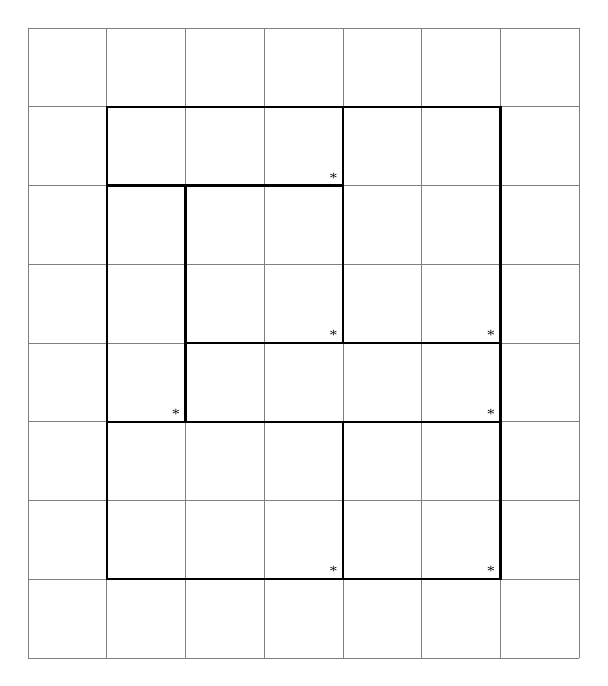
\begin{tikzpicture}

% define base units ------------------------------------------------------------
	\def\delta{1/10}

% draw grid --------------------------------------------------------------------
	\draw[step=1, gray, very thin] (-1,-1) grid (6,7);

% draw rectangles --------------------------------------------------------------
	\def\rect{
%		coord_x / coord_y / size_x /size_y
		0 / 0 / 3 / 2,
		0 / 2 / 1 / 3,
		0 / 5 / 3 / 1,
		1 / 2 / 4 / 1,
		1 / 3 / 2 / 2,
		3 / 0 / 2 / 2,
		3 / 3 / 2 / 3
	}
	\foreach \x / \y / \sx / \sy in \rect
	{
		\draw[thick] (\x,\y) rectangle +(\sx,\sy);
		\node[shift={(\x+\sx-1.2\delta,\y+1.2\delta)}] {\tiny\(\ast\)};
	}

\end{tikzpicture}
